\documentclass{article}

\usepackage[acronym,toc]{glossaries}
%\newacronym{<++>}{<++>}{<++>}
\newacronym[longplural={metric tons of heavy metal}]{MTHM}{MTHM}{metric ton of heavy metal}
\newacronym{ABM}{ABM}{agent-based modeling}
\newacronym{ACDIS}{ACDIS}{Program in Arms Control \& Domestic and International Security}
\newacronym{AHTR}{AHTR}{Advanced High Temperature Reactor}
\newacronym{ANDRA}{ANDRA}{Agence Nationale pour la gestion des D\'echets RAdioactifs, the French National Agency for Radioactive Waste Management}
\newacronym{ANL}{ANL}{Argonne National Laboratory}
\newacronym{ANS}{ANS}{American Nuclear Society}
\newacronym{API}{API}{application programming interface}
\newacronym{ARE}{ARE}{Aircraft Reactor Experiment}
\newacronym{ARFC}{ARFC}{Advanced Reactors and Fuel Cycles}
\newacronym{ASME}{ASME}{American Society of Mechanical Engineers}
\newacronym{ATWS}{ATWS}{Anticipated Transient Without Scram}
\newacronym{BDBE}{BDBE}{Beyond Design Basis Event}
\newacronym{BIDS}{BIDS}{Berkeley Institute for Data Science}
\newacronym{CAFCA}{CAFCA}{ Code for Advanced Fuel Cycles Assessment }
\newacronym{CDTN}{CDTN}{Centro de Desenvolvimento da Tecnologia Nuclear}
\newacronym{CEA}{CEA}{Commissariat \`a l'\'Energie Atomique et aux \'Energies Alternatives}
\newacronym{CFD}{CFD}{Computational Fluid Dynamics}
\newacronym{CI}{CI}{continuous integration}
\newacronym{CNEN}{CNEN}{Comiss\~{a}o Nacional de Energia Nuclear}
\newacronym{CNERG}{CNERG}{Computational Nuclear Engineering Research Group}
\newacronym{COSI}{COSI}{Commelini-Sicard}
\newacronym{COTS}{COTS}{commercial, off-the-shelf}
\newacronym{CSNF}{CSNF}{commercial spent nuclear fuel}
\newacronym{CTAH}{CTAHs}{Coiled Tube Air Heaters}
\newacronym{CUBIT}{CUBIT}{CUBIT Geometry and Mesh Generation Toolkit}
\newacronym{CURIE}{CURIE}{Centralized Used Fuel Resource for Information Exchange}
\newacronym{DAG}{DAG}{directed acyclic graph}
\newacronym{DANESS}{DANESS}{Dynamic Analysis of Nuclear Energy System Strategies}
\newacronym{DBE}{DBE}{Design Basis Event}
\newacronym{DESAE}{DESAE}{Dynamic Analysis of Nuclear Energy Systems Strategies}
\newacronym{DHS}{DHS}{Department of Homeland Security}
\newacronym{DOE}{DOE}{Department of Energy}
\newacronym{DRACS}{DRACS}{Direct Reactor Auxiliary Cooling System}
\newacronym{DRE}{DRE}{dynamic resource exchange}
\newacronym{DSNF}{DSNF}{DOE spent nuclear fuel}
\newacronym{DYMOND}{DYMOND}{Dynamic Model of Nuclear Development }
\newacronym{EBS}{EBS}{Engineered Barrier System}
\newacronym{EDF}{EDF}{Électricité de France}
\newacronym{EDZ}{EDZ}{Excavation Disturbed Zone}
\newacronym{EIA}{EIA}{U.S. Energy Information Administration}
\newacronym{EPA}{EPA}{Environmental Protection Agency}
\newacronym{EPR}{EPR}{European Pressurized Reactors}
\newacronym{EP}{EP}{Engineering Physics}
\newacronym{EU}{EU}{European Union}
\newacronym{FCO}{FCO}{Fuel Cycle Options}
\newacronym{FCT}{FCT}{Fuel Cycle Technology}
\newacronym{FEHM}{FEHM}{Finite Element Heat and Mass Transfer}
\newacronym{FEPs}{FEPs}{Features, Events, and Processes}
\newacronym{FHR}{FHR}{Fluoride-Salt-Cooled High-Temperature Reactor}
\newacronym{FLiBe}{FLiBe}{Fluoride-Lithium-Beryllium}
\newacronym{FP}{FP}{Fission Product}
\newacronym{GDSE}{GDSE}{Generic Disposal System Environment}
\newacronym{GDSM}{GDSM}{Generic Disposal System Model}
\newacronym{GENIUSv1}{GENIUSv1}{Global Evaluation of Nuclear Infrastructure Utilization Scenarios, Version 1}
\newacronym{GENIUSv2}{GENIUSv2}{Global Evaluation of Nuclear Infrastructure Utilization Scenarios, Version 2}
\newacronym{GENIUS}{GENIUS}{Global Evaluation of Nuclear Infrastructure Utilization Scenarios}
\newacronym{GIF}{GIF}{Generation IV International Forum}
\newacronym{GPAM}{GPAM}{Generic Performance Assessment Model}
\newacronym{GRSAC}{GRSAC}{Graphite Reactor Severe Accident Code}
\newacronym{GUI}{GUI}{graphical user interface}
\newacronym{HLW}{HLW}{high level waste}
\newacronym{HPC}{HPC}{high-performance computing}
\newacronym{HTC}{HTC}{high-throughput computing}
\newacronym{HTGR}{HTGR}{High Temperature Gas-Cooled Reactor}
\newacronym{IAEA}{IAEA}{International Atomic Energy Agency}
\newacronym{IEMA}{IEMA}{Illinois Emergency Mangament Agency}
\newacronym{IHLRWM}{IHLRWM}{International High Level Radioactive Waste Management}
\newacronym{INL}{INL}{Idaho National Laboratory}
\newacronym{IPRR1}{IRP-R1}{Instituto de Pesquisas Radioativas Reator 1}
\newacronym{IRP}{IRP}{Integrated Research Project}
\newacronym{ISFSI}{ISFSI}{Independent Spent Fuel Storage Installation}
\newacronym{ISRG}{ISRG}{Independent Student Research Group}
\newacronym{JFNK}{JFNK}{Jacobian-Free Newton Krylov}
\newacronym{LANL}{LANL}{Los Alamos National Laboratory}
\newacronym{LBNL}{LBNL}{Lawrence Berkeley National Laboratory}
\newacronym{LCOE}{LCOE}{levelized cost of electricity}
\newacronym{LDRD}{LDRD}{laboratory directed research and development}
\newacronym{LFR}{LFR}{Lead-Cooled Fast Reactor}
\newacronym{LLNL}{LLNL}{Lawrence Livermore National Laboratory}
\newacronym{LMFBR}{LMFBR}{Liquid Metal Fast Breeder Reactor}
\newacronym{LOFC}{LOFC}{Loss of Forced Cooling}
\newacronym{LOHS}{LOHS}{Loss of Heat Sink}
\newacronym{LOLA}{LOLA}{Loss of Large Area}
\newacronym{LP}{LP}{linear program}
\newacronym{LWR}{LWR}{Light Water Reactor}
\newacronym{MAGNOX}{MAGNOX}{Magnesium Alloy Graphie Moderated Gas Cooled Uranium Oxide Reactor}
\newacronym{MA}{MA}{minor actinide}
\newacronym{MCNP}{MCNP}{Monte Carlo N-Particle code}
\newacronym{MILP}{MILP}{mixed-integer linear program}
\newacronym{MIT}{MIT}{the Massachusetts Institute of Technology}
\newacronym{MOAB}{MOAB}{Mesh-Oriented datABase}
\newacronym{MOOSE}{MOOSE}{Multiphysics Object-Oriented Simulation Environment}
\newacronym{MOSART}{MOSART}{Molten Salt Actinide Recycler and Transmuter}
\newacronym{MOX}{MOX}{mixed oxide}
\newacronym{MPI}{MPI}{Message Passing Interface}
\newacronym{MRPP}{MRPP}{Multiregion Processing Plant}
\newacronym{MSBR}{MSBR}{Molten Salt Breeder Reactor}
\newacronym{MSFR}{MSFR}{Molten Salt Fast Reactor}
\newacronym{MSRE}{MSRE}{Molten Salt Reactor Experiment}
\newacronym{MSR}{MSR}{Molten Salt Reactor}
\newacronym{NAGRA}{NAGRA}{National Cooperative for the Disposal of Radioactive Waste}
\newacronym{NEAMS}{NEAMS}{Nuclear Engineering Advanced Modeling and Simulation}
\newacronym{NEUP}{NEUP}{Nuclear Energy University Programs}
\newacronym{NFCSim}{NFCSim}{Nuclear Fuel Cycle Simulator}
\newacronym{NGNP}{NGNP}{Next Generation Nuclear Plant}
\newacronym{NMWPC}{NMWPC}{Nuclear MW Per Capita}
\newacronym{NNSA}{NNSA}{National Nuclear Security Administration}
\newacronym{NPP}{NPP}{Nuclear Power Plant}
\newacronym{NPRE}{NPRE}{Department of Nuclear, Plasma, and Radiological Engineering}
\newacronym{NQA1}{NQA-1}{Nuclear Quality Assurance - 1}
\newacronym{NRC}{NRC}{Nuclear Regulatory Commission}
\newacronym{NSF}{NSF}{National Science Foundation}
\newacronym{NSSC}{NSSC}{Nuclear Science and Security Consortium}
\newacronym{NUWASTE}{NUWASTE}{Nuclear Waste Assessment System for Technical Evaluation}
\newacronym{NWF}{NWF}{Nuclear Waste Fund}
\newacronym{NWTRB}{NWTRB}{Nuclear Waste Technical Review Board}
\newacronym{OCRWM}{OCRWM}{Office of Civilian Radioactive Waste Management}
\newacronym{ORION}{ORION}{ORION}
\newacronym{ORNL}{ORNL}{Oak Ridge National Laboratory}
\newacronym{PARCS}{PARCS}{Purdue Advanced Reactor Core Simulator}
\newacronym{PBAHTR}{PB-AHTR}{Pebble Bed Advanced High Temperature Reactor}
\newacronym{PBFHR}{PB-FHR}{Pebble-Bed Fluoride-Salt-Cooled High-Temperature Reactor}
\newacronym{PEI}{PEI}{Peak Environmental Impact}
\newacronym{PH}{PRONGHORN}{PRONGHORN}
\newacronym{PRIS}{PRIS}{Power Reactor Information System}
\newacronym{PRKE}{PRKE}{Point Reactor Kinetics Equations}
\newacronym{PSPG}{PSPG}{Pressure-Stabilizing/Petrov-Galerkin}
\newacronym{PWAR}{PWAR}{Pratt and Whitney Aircraft Reactor}
\newacronym{PWR}{PWR}{Pressurized Water Reactor}
\newacronym{PyNE}{PyNE}{Python toolkit for Nuclear Engineering}
\newacronym{PyRK}{PyRK}{Python for Reactor Kinetics}
\newacronym{QA}{QA}{quality assurance}
\newacronym{RDD}{RD\&D}{Research Development and Demonstration}
\newacronym{RD}{R\&D}{Research and Development}
\newacronym{REE}{REE}{rare earth element}
\newacronym{RELAP}{RELAP}{Reactor Excursion and Leak Analysis Program}
\newacronym{RIA}{RIA}{Reactivity Insertion Accident}
\newacronym{RIF}{RIF}{Region-Institution-Facility}
\newacronym{ROD}{ROD}{Reactor Optimum Design}
\newacronym{SFR}{SFR}{Sodium-Cooled Fast Reactor}
\newacronym{SINDAG}{SINDA{\textbackslash}G}{Systems Improved Numerical Differencing Analyzer $\backslash$ Gaski}
\newacronym{SKB}{SKB}{Svensk K\"{a}rnbr\"{a}nslehantering AB}
\newacronym{SNF}{SNF}{spent nuclear fuel}
\newacronym{SNL}{SNL}{Sandia National Laboratory}
\newacronym{STC}{STC}{specific temperature change}
\newacronym{SUPG}{SUPG}{Streamline-Upwind/Petrov-Galerkin}
\newacronym{SWF}{SWF}{Separations and Waste Forms}
\newacronym{SWU}{SWU}{Separative Work Unit}
\newacronym{TRIGA}{TRIGA}{Training Research Isotope General Atomic}
\newacronym{TRISO}{TRISO}{Tristructural Isotropic}
\newacronym{TSM}{TSM}{Total System Model}
\newacronym{TSPA}{TSPA}{Total System Performance Assessment for the Yucca Mountain License Application}
\newacronym{ThOX}{ThOX}{thorium oxide}
\newacronym{UDB}{UDB}{Unified Database}
\newacronym{UFD}{UFD}{Used Fuel Disposition}
\newacronym{UML}{UML}{Unified Modeling Language}
\newacronym{UNFSTANDARDS}{UNFST\&DARDS}{Used Nuclear Fuel Storage, Transportation \& Disposal Analysis Resource and Data System}
\newacronym{UNF}{UNF}{used nuclear fuel}
\newacronym{UOX}{UOX}{uranium oxide}
\newacronym{UQ}{UQ}{uncertainty quantification}
\newacronym{US}{US}{United States}
\newacronym{UW}{UW}{University of Wisconsin}
\newacronym{VISION}{VISION}{the Verifiable Fuel Cycle Simulation Model}
\newacronym{VVER}{VVER}{Voda-Vodyanoi Energetichesky Reaktor (Russian Pressurized Water Reactor)}
\newacronym{VV}{V\&V}{verification and validation}
\newacronym{WIPP}{WIPP}{Waste Isolation Pilot Plant}
\newacronym{YMR}{YMR}{Yucca Mountain Repository Site}


\makeglossaries


\usepackage{lineno}
\usepackage{xspace}

%%%% packages and definitions (optional)
\usepackage{placeins}
\usepackage{booktabs} % nice rules (thick lines) for tables
\usepackage{microtype} % improves typography for PDF
\usepackage{hhline}
\usepackage{amsmath}

%\usepackage[demo]{graphicx}
%\usepackage{caption}
%\usepackage{subcaption}

\usepackage{booktabs}
\usepackage{threeparttable, tablefootnote}

\usepackage{tabularx}
\newcolumntype{b}{>{\hsize=1.0\hsize}X}
\newcolumntype{s}{>{\hsize=.5\hsize}X}
\newcolumntype{m}{>{\hsize=.75\hsize}X}
\newcolumntype{x}{>{\hsize=.25\hsize}X}


% tikz %
\usepackage{tikz}
\usetikzlibrary{positioning, arrows, decorations, shapes}

\usetikzlibrary{shapes.geometric,arrows}
\tikzstyle{process} = [rectangle, rounded corners, minimum width=3cm, minimum height=1cm,text centered, draw=black, fill=blue!30]
\tikzstyle{object} = [ellipse, rounded corners, minimum width=3cm, minimum height=1cm,text centered, draw=black, fill=green!30]
\tikzstyle{arrow} = [thick,->,>=stealth]

% Cyclus
\newcommand{\Cyclus}{\textsc{Cyclus}\xspace}%

% hyperref %
\usepackage[hidelinks]{hyperref}

\begin{document}
\title{Workshopping Figures and Visualizations}
\author{Kathryn D. Huff$^{1}$\\
        $^{1}$Dept. of Nuclear, Plasma, and Radiological Engineering, \\
University of Illinois at Urbana-Champaign, \\
Urbana, IL}

\date{}
\maketitle 
These plots resulted from the hard work of three graduate students in the 
Advanced Reactors and Fuel Cycles group: Jin Whan Bae, Gwendolyn 
Chee, and Andrei Rykhlevskii.

\section*{Recycling Fuel in a Molten Salt Breeder Reactor \cite{rykhlevskii_modeling_2018}}

\textbf{PhD student Andrei Rykhlevskii ran long-time-scale, 
        high-geometric-fidelity  depletion (neutron 
transport) and online reprocessing (fancy chemistry) calculations to determine 
the equilibrium composition of the nuclear fuel and other characteristics in a 
particular molten salt reactor design from the 70s.} 

Figure~\ref{fig:pow_den} reflects the
normalized power distribution of the \gls{MSBR} quarter core, which is the same
at both the initial and equilibrium states. For both the initial and equilibrium compositions, fission
primarily occurs in the center of the core, namely zone I. The spectral shift
during reactor operation results in different power fractions at startup and
equilibrium, but most of the power is still generated in zone I at equilibrium.

Figure~\ref{fig:breeding_den} shows the neutron capture reaction rate
distribution for $^{232}$Th normalized by the total neutron flux for initial
and equilibrium states. The distribution reflects the spatial distribution of
$^{233}$Th production in the core. The thorium-232 then $\beta$-decays to
$^{233}$Pa, which is the precursor for $^{233}$U production. Accordingly, this
characteristic represents the breeding distribution in the \gls{MSBR} core.
Spectral shift does not cause significant changes in power nor in breeding
distribution. Even after 20 years of operation, most of the power is still
generated in zone I and the majority of $^{233}$Th is
produced in zone II.

\begin{figure}[ht!] % replace 't' with 'b' to force it to \centering
  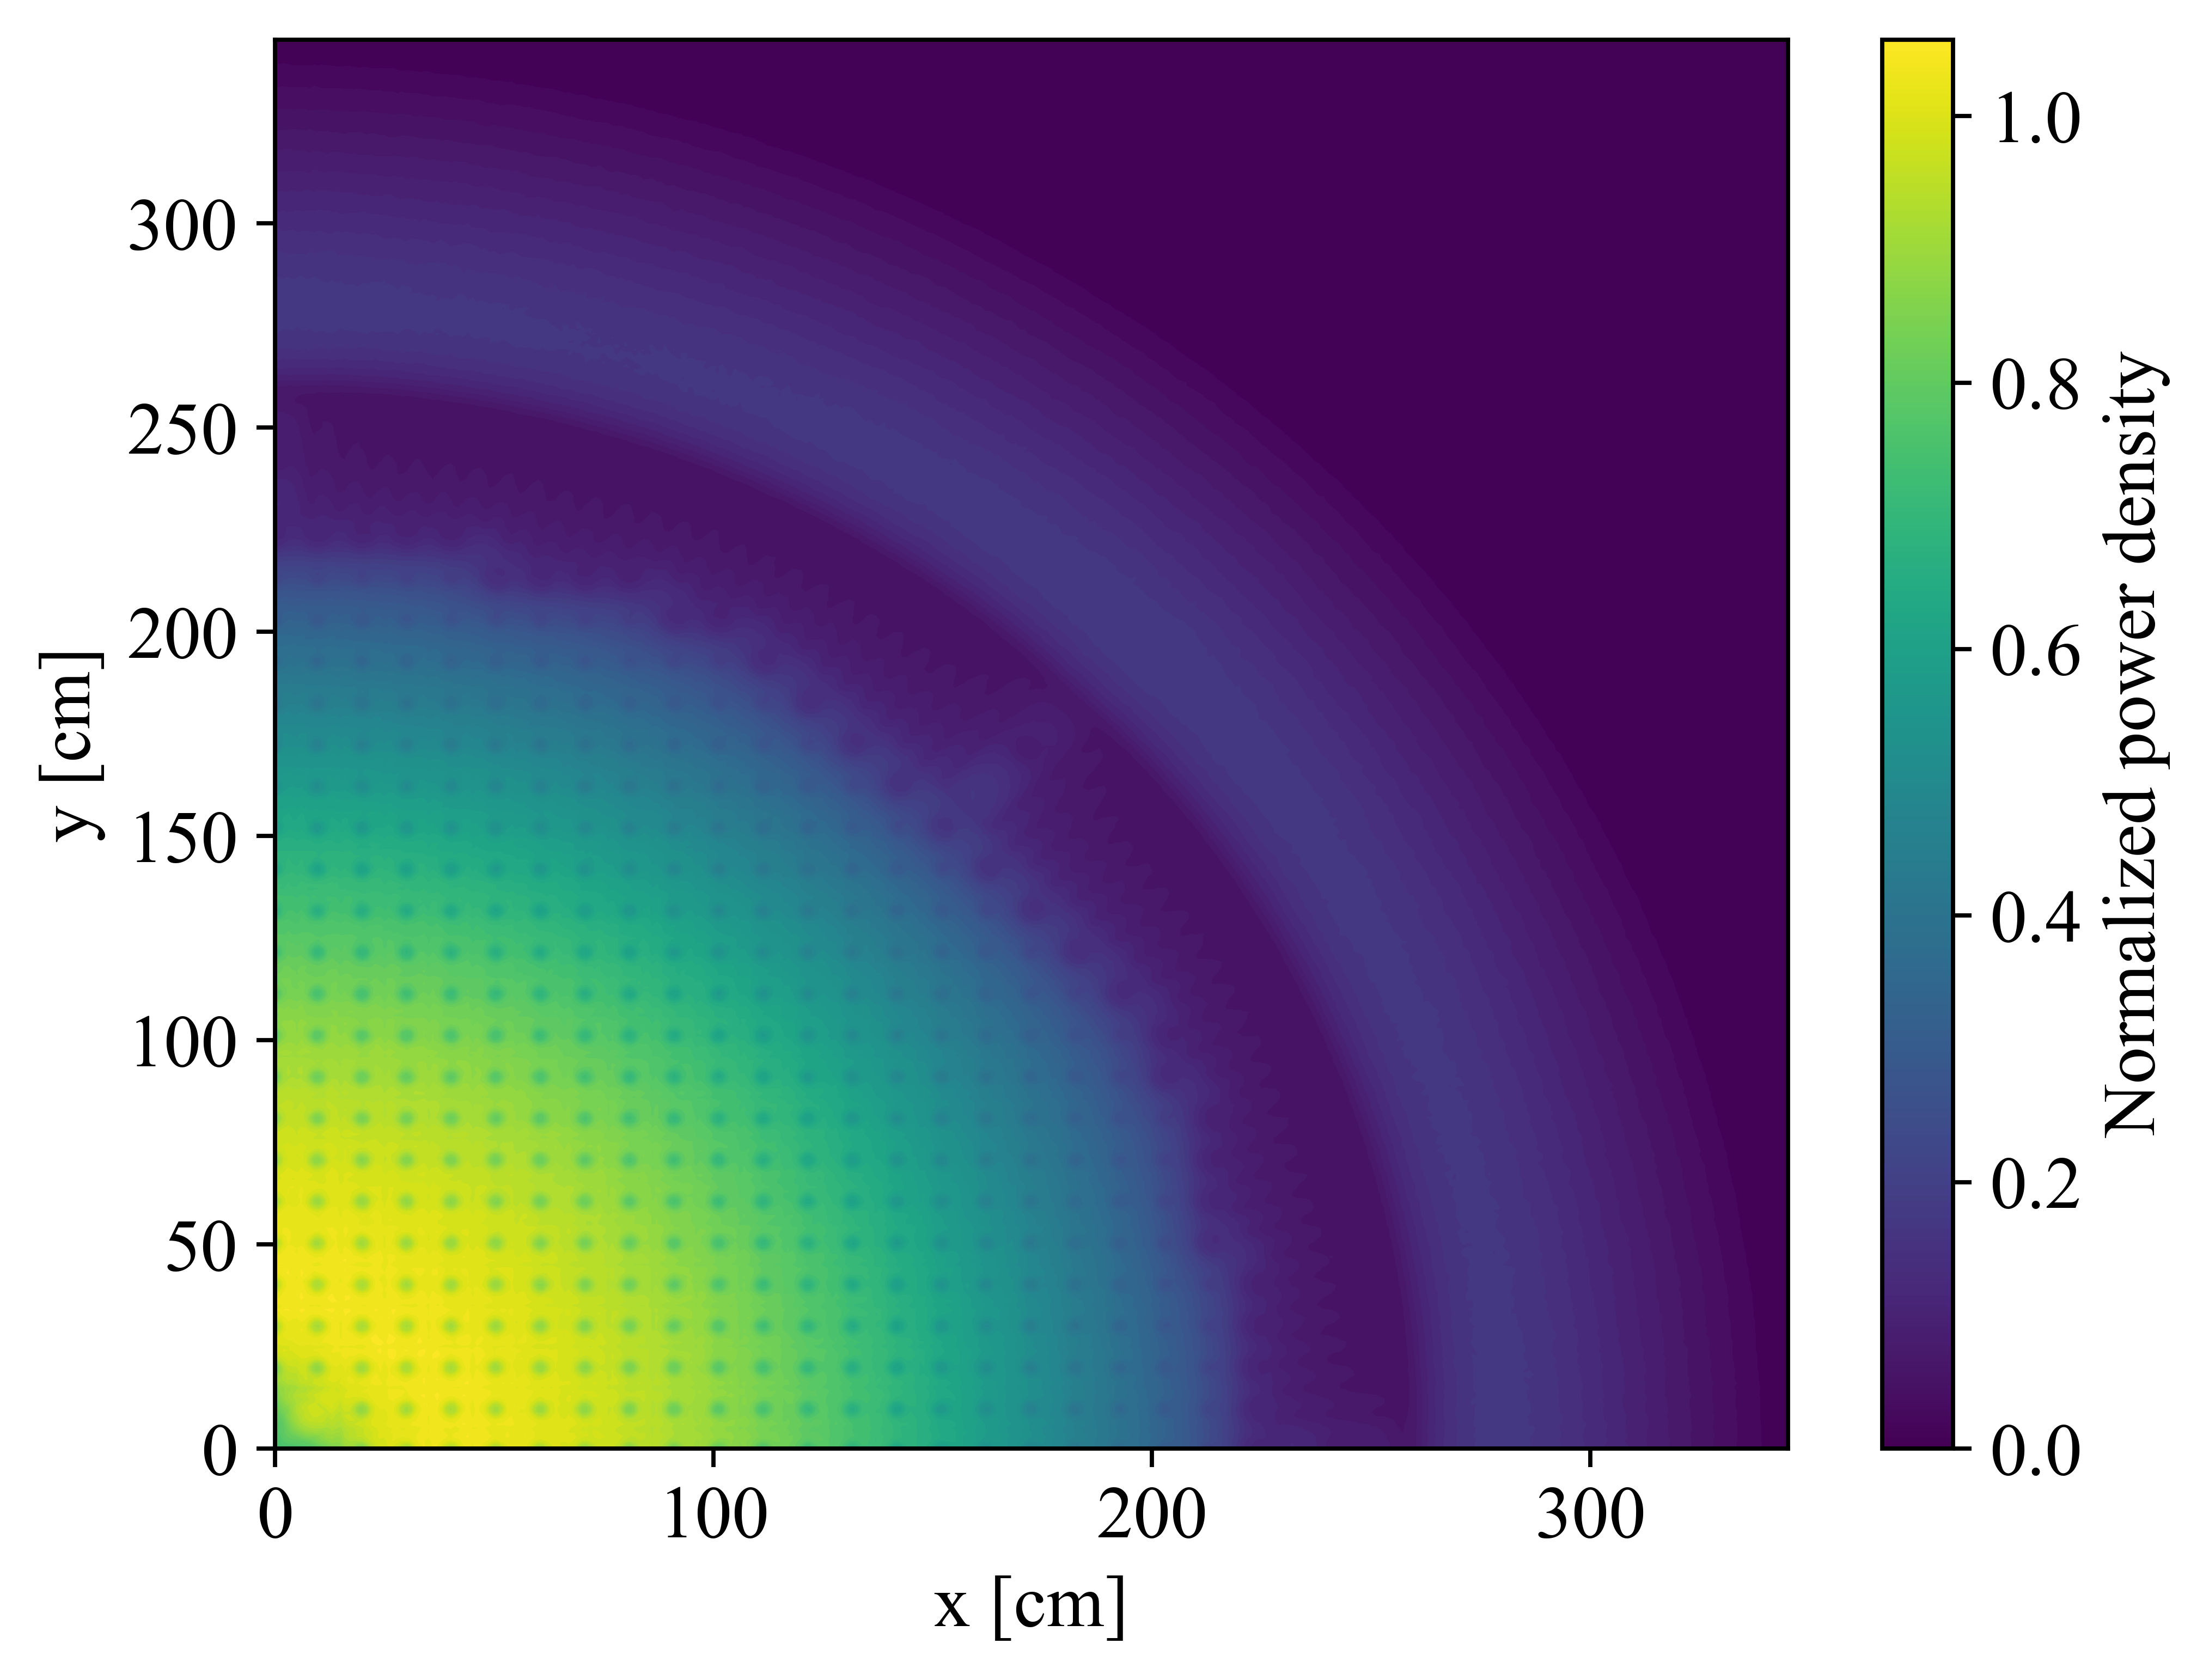
\includegraphics[width=\textwidth]{power_distribution_eq.png}
  \caption{Normalized power density for equilibrium fuel salt
  composition.}
  \label{fig:pow_den}
\end{figure}
\begin{figure}[ht!] % replace 't' with 'b' to force it to \centering
  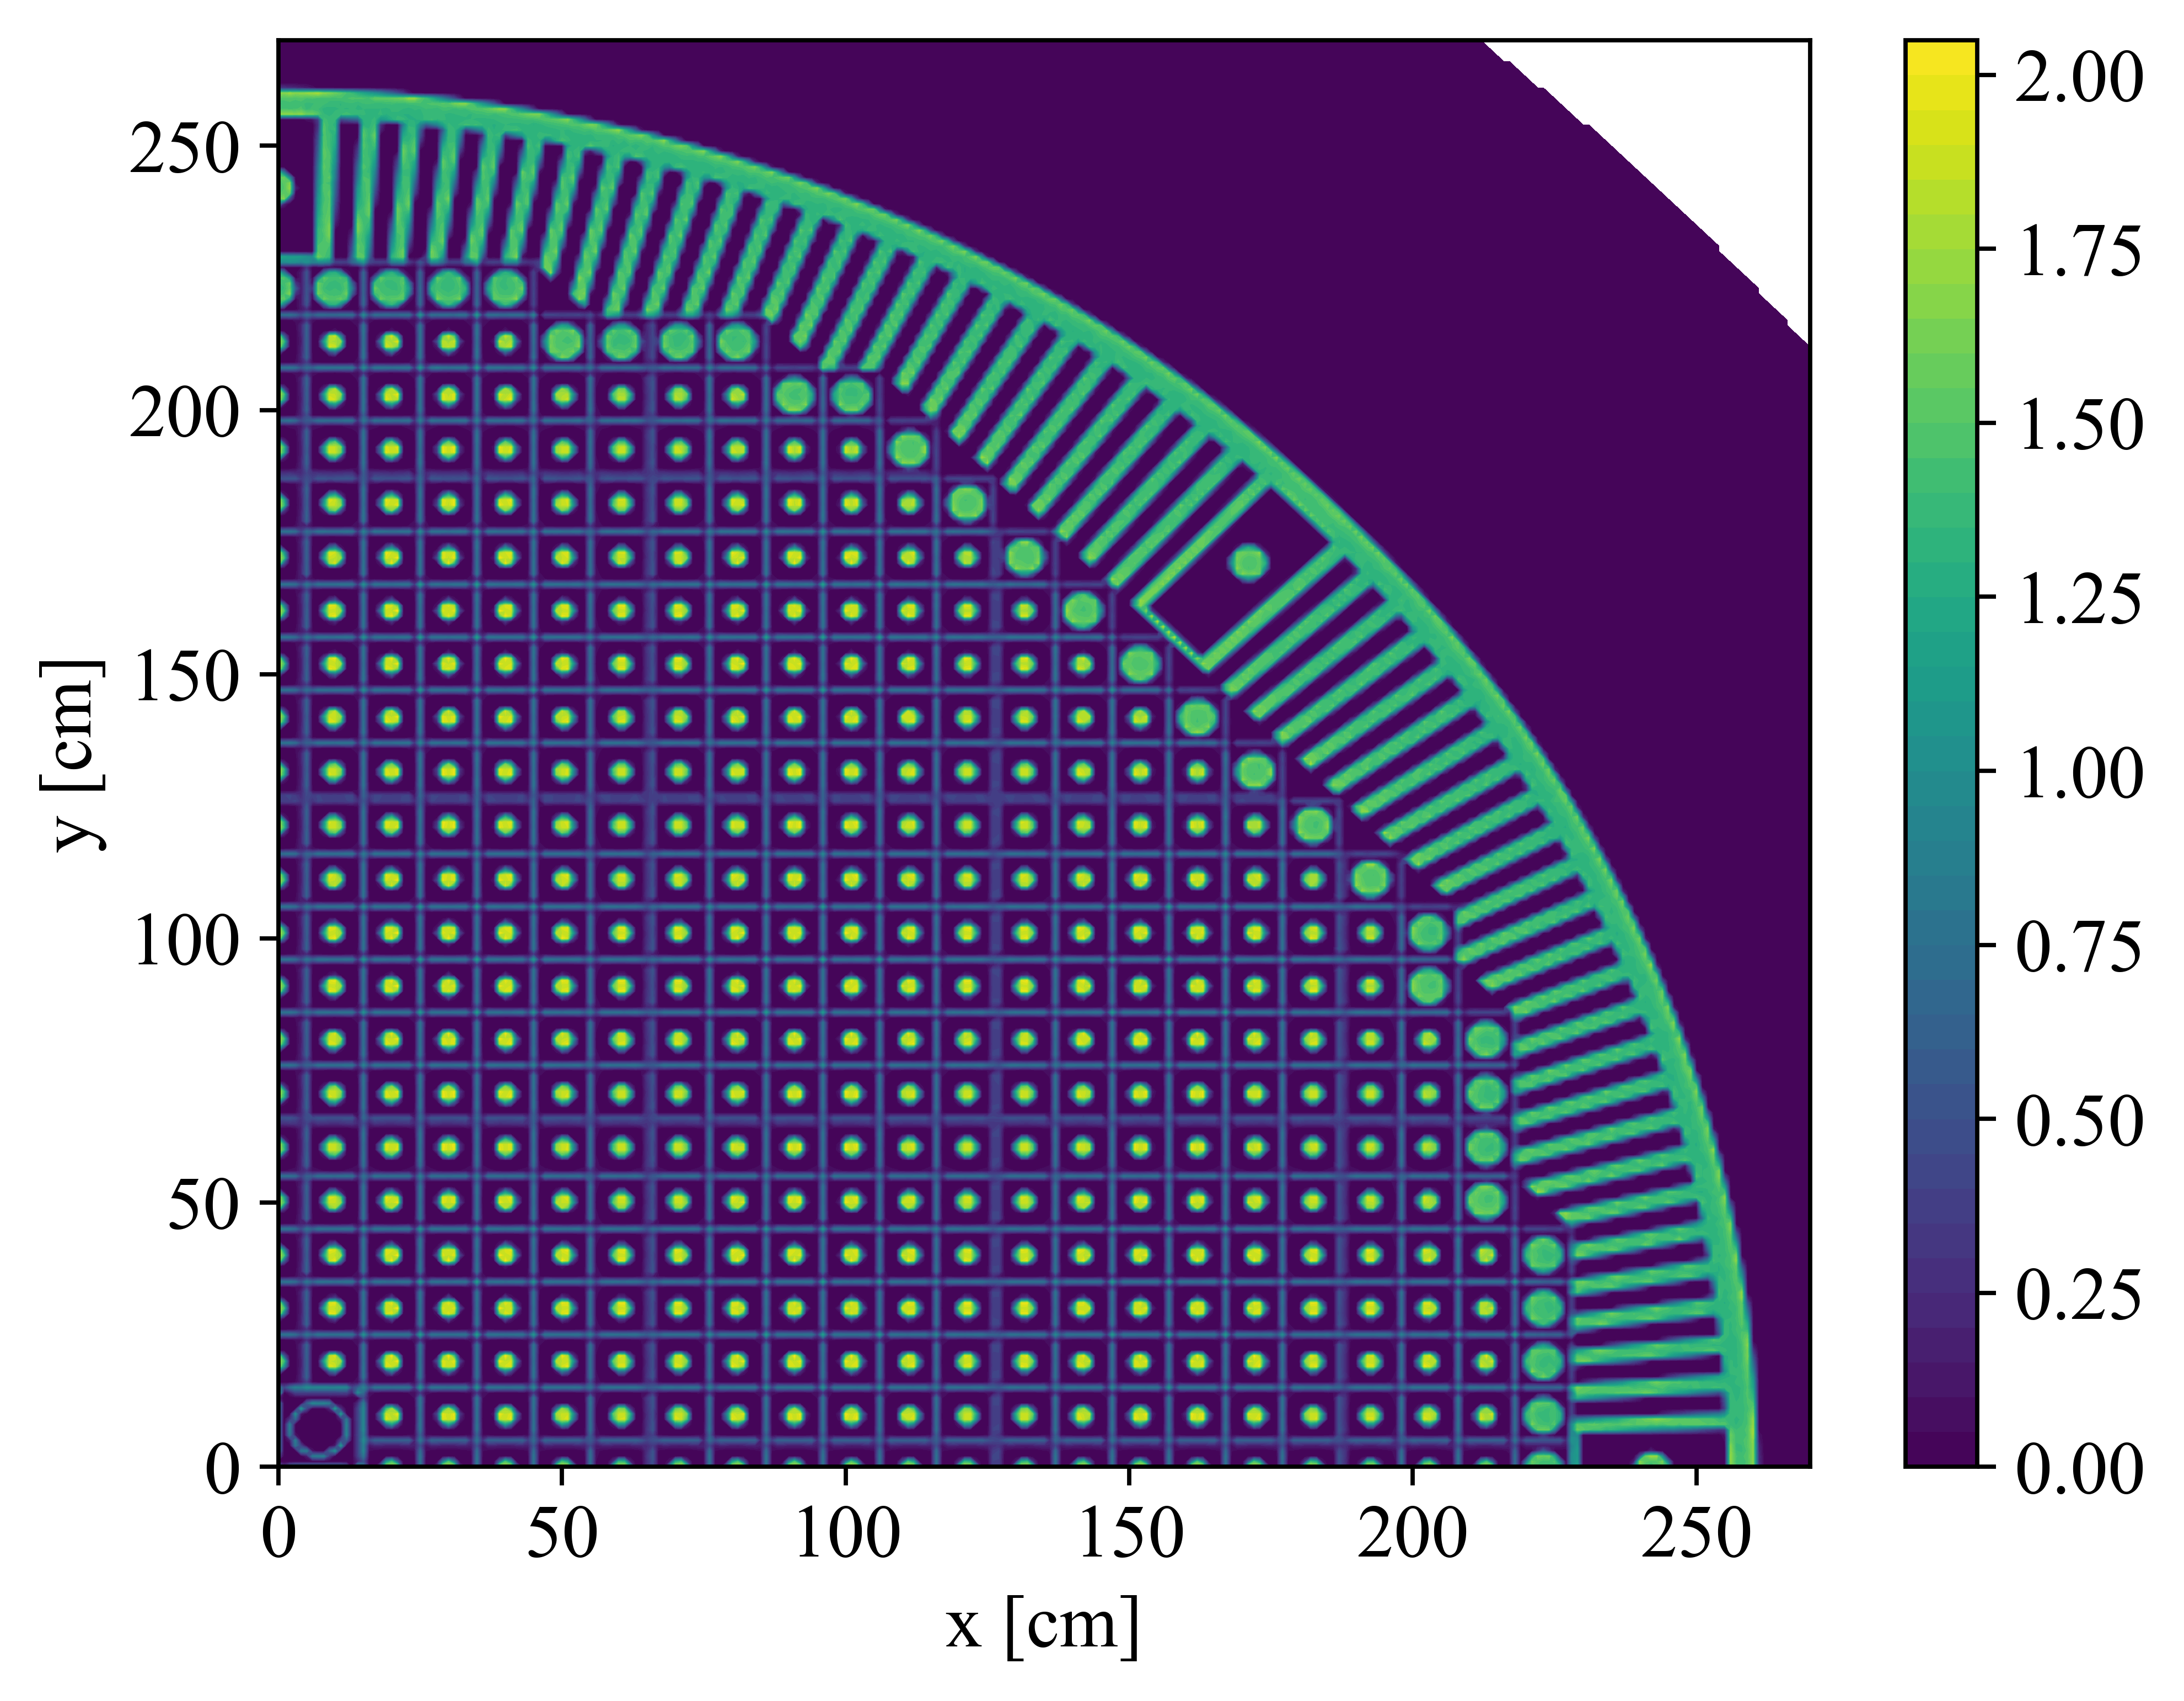
\includegraphics[width=\textwidth]{breeding_distribution_eq.png}
  \caption{$^{232}$Th neutron capture reaction rate normalized by total flux
  for equilibrium fuel salt composition.}
  \label{fig:breeding_den}
\end{figure}

In a \gls{MSBR} reprocessing scheme, the only external feed material flow  is
$^{232}$Th. Figure~\ref{fig:th_refill} shows the $^{232}$Th feed rate
calculated for 60 years of reactor operation. The $^{232}$Th feed rate
fluctuates significantly as a result of the batch-wise nature of this online
reprocessing approach. For example, the large spikes of up to 36 kg/day in a
thorium consumption occurs every 3435 days. This is required due to batch-wise
removal of strong absorbers (Rb, Sr, Cs, Ba). The corresponding effective
multiplication factor increase and breeding
intensification leads to additional $^{232}$Th consumption.

\begin{figure}[ht!] % replace 't' with 'b' to force it to \centering
  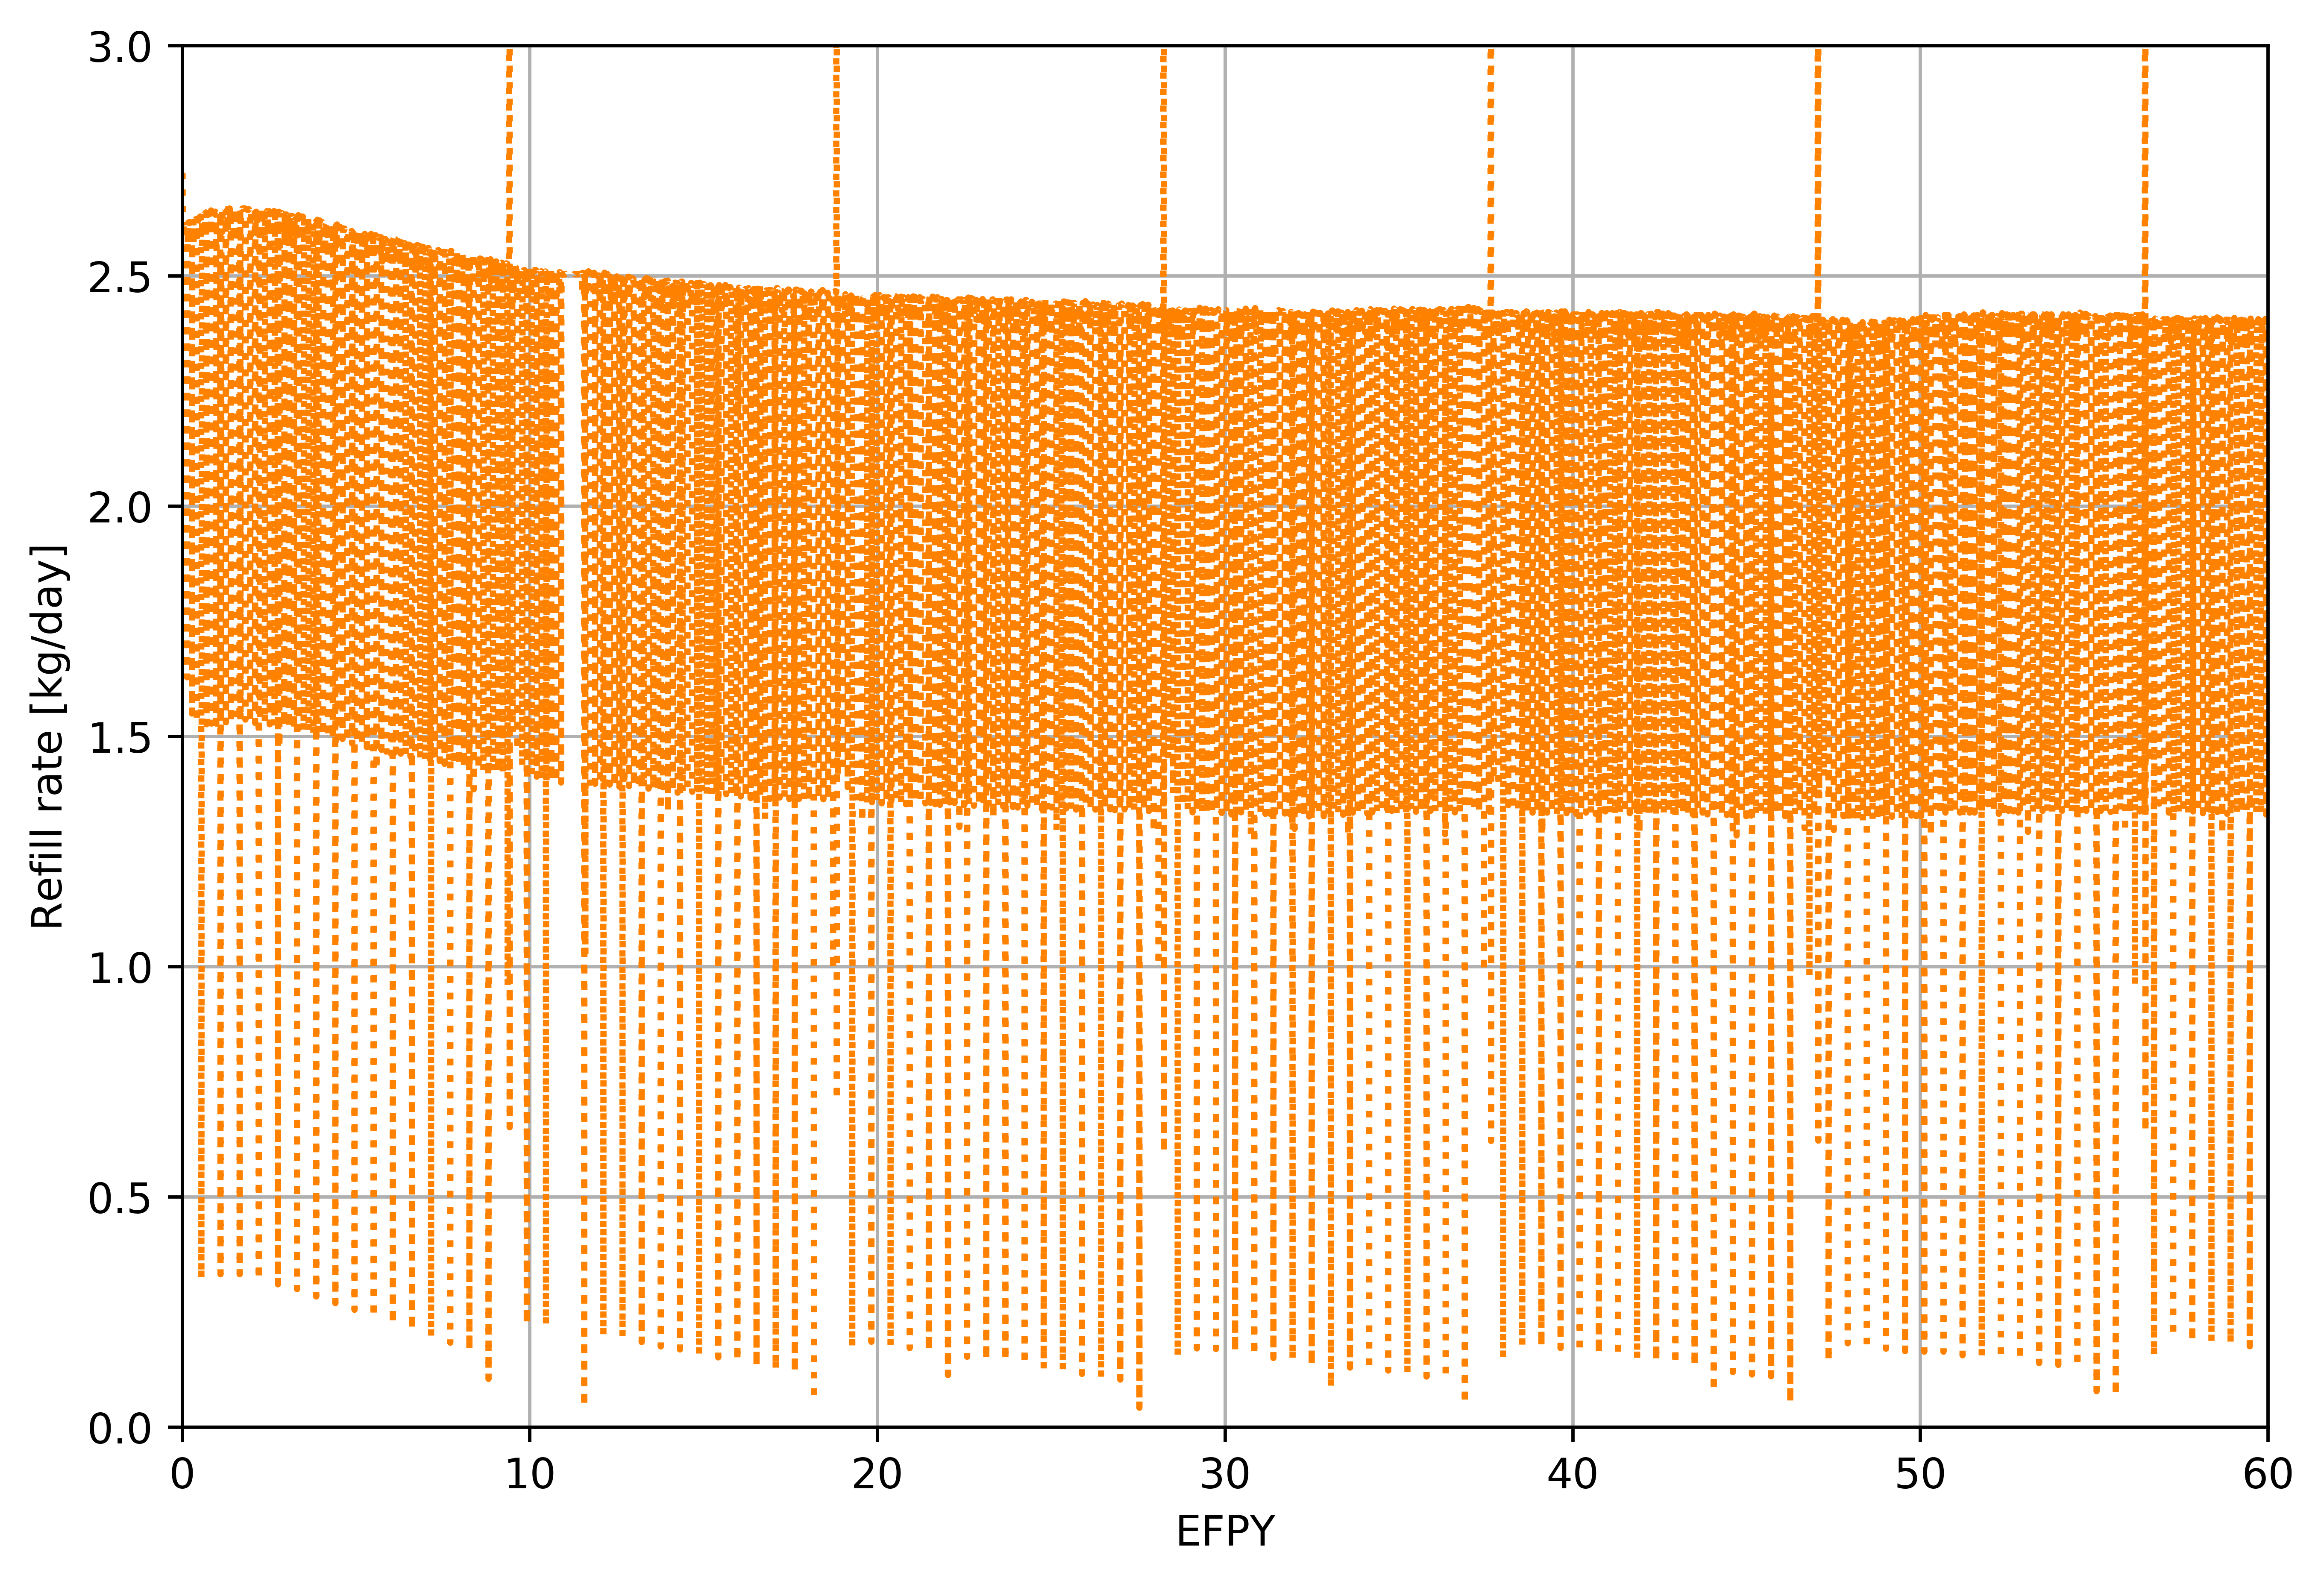
\includegraphics[width=\textwidth]{Th_refill_rate.png} \caption{$^{232}$Th
  feed rate over 60 years of \gls{MSBR} operation.}
  \label{fig:th_refill}
\end{figure}

\FloatBarrier
\section*{Benchmarking : Agent-Based Simulation more Informative than Spreadsheets \cite{bae_standardized_2018}}
\textbf{MS student Jin Whan Bae compared an agent based fuel cycle simulator 
        with estimates from a spreadsheet (via DOE). The rich, discrete 
        facility and discrete material information available from the agent 
based simulation captures dynamics that the benchmark was forced to approximate 
at the fleet level.}

A code-to-code benchmarking exercise postulated a nuclear fuel cycle transition 
from current reactors to new ones. 
Figure \ref{fig:waiting_monthly} shows the amount of cooled \gls{UNF} waiting 
for
reprocessing. The value is calculated by subtracting the cumulative difference 
between
the cooled inventory and the \gls{UNF} reprocessing throughput.
The oscillation is between the cooled inventory in the storage facility before 
(high)
and after (low) it sends its inventory for reprocessing.

Figure \ref{fig:rep} shows the reprocessing throughput, which oscillates around
the benchmark solution. No oscillation exists in the beginning because the
\gls{LWR} \gls{UNF} reprocessing plant throughput peaks at 2,000 tons per year.


\begin{figure}[htbp!]
    \begin{center}
            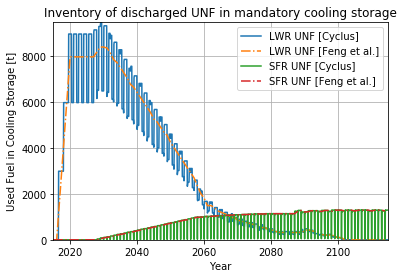
\includegraphics[width=\textwidth]{./fuel_discharge_monthly.png}
    \end{center}
        \caption{Inventory of discharged \gls{UNF} in mandatory cooling storage.}
    \label{fig:fuel_discharge_monthly}
\end{figure}


\begin{figure}[htbp!]
    \begin{center}
            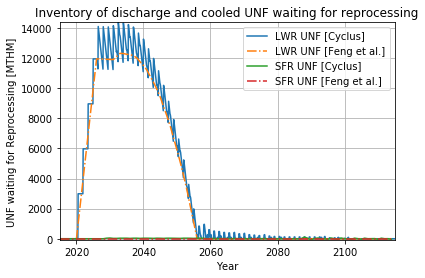
\includegraphics[width=\textwidth]{./waiting_monthly.png}
    \end{center}
        \caption{Inventory of discharged and cooled \gls{UNF} waiting for reprocessing.}
    \label{fig:waiting_monthly}
\end{figure}


\begin{figure}[htbp!]
    \begin{center}
            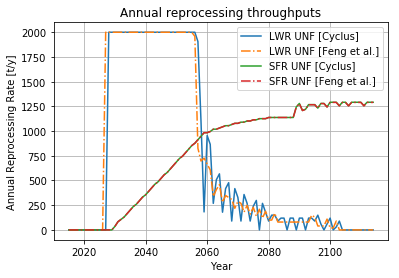
\includegraphics[width=\textwidth]{./rep.png}
    \end{center}
        \caption{Annual reprocessing throughputs.}
    \label{fig:rep}
\end{figure}

\FloatBarrier
\section*{Validating a Predictive Simulator by Predicting the Past \cite{chee_validation_2018}}

\textbf{PhD student Gwendolyn Chee sought to validate our predictive nuclear 
fuel cycle simulator by predicting the past. That is, she set up a simulation 
with initial conditions reflecting our US nuclear reactor fleet and used the 
Cyclus simulator to determine the cumulative isotopics of US spent fuel over 
the last many decades. She compared this to a database holding the DOE's best 
guess (using high fidelity calculations of each reactor) at the same data.}

Figures \ref{fig:absolute_diff_all_51} and \ref{fig:absolute_diff_all_33} show
the cumulative nuclear spent fuel isotopic mass difference between \gls{UNFSTANDARDS} 
\gls{UDB} and simulated \Cyclus data
in 5 year intervals for burnup of 51 GWD/MTU and 33 GWD/MTU correspondingly.
The \Cyclus data that assumed 33 GWD/MTU burnup deviated less than the
\Cyclus data that assumed 51 GWD/MTU burnup. This is apparent for $^{236}$U,
$^{242}$Pu and $^{240}$Pu. They are similar for the isotopes on the left side
of both figures. With an exception of $^{239}$Pu having a substantially larger
difference for 33 GWD/MTU than 51 GWD/MTU.

\begin{figure}[htb] % replace 't' with 'b' to force it to be on the bottom
    \centering
        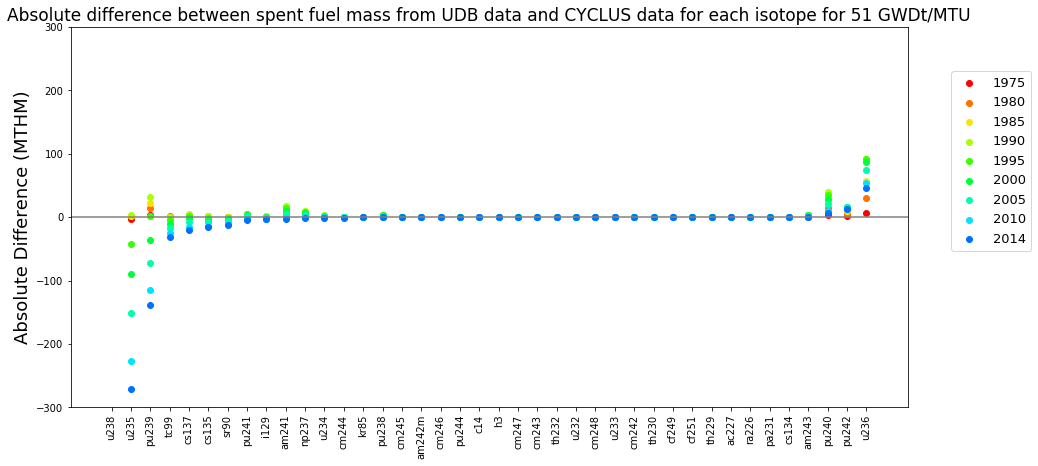
\includegraphics[height=0.30\textheight]{absolute_diff_all_51}
        \caption{The absolute difference between spent fuel mass calculated by 
        \gls{UNFSTANDARDS} \gls{UDB} and \Cyclus for each isotope for 51 GWD/MTU burnup. Positive difference indicates \Cyclus mass estimate is larger.}
    \label{fig:absolute_diff_all_51}
\end{figure}

\begin{figure}[htb] % replace 't' with 'b' to force it to be on the bottom
        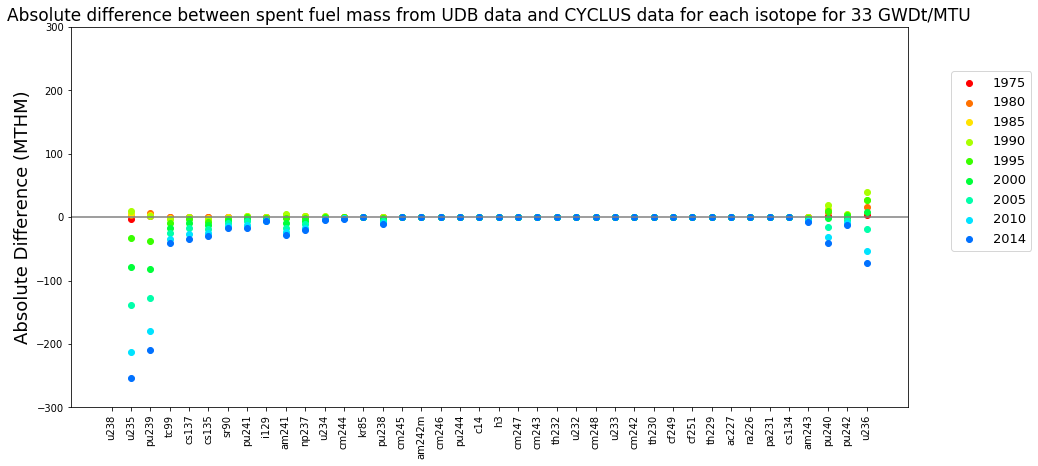
\includegraphics[height=0.30\textheight]{absolute_diff_all_33}
        \caption{The absolute difference between spent fuel mass calculated by \gls{UNFSTANDARDS} \gls{UDB} and \Cyclus for each isotope for 33 GWD/MTU burnup. Positive difference indicates \Cyclus mass estimate is larger.}
    \label{fig:absolute_diff_all_33}
\end{figure}



\FloatBarrier
%%%%%%%%%%%%%%%%%%%%%%%%%%%%%%%%%%%%%%%%%%%%%%%%%%%%%%%%%%%%%%%%%%%%%%%%%%%%%%%%
\bibliographystyle{plain}
\bibliography{2018-huff-msdseviz}
\end{document}
